% import macros and common styles
\documentclass[11pt]{article}
\usepackage[margin=1in]{geometry}
\usepackage{fancyhdr}
\usepackage[noindentafter]{titlesec}
\usepackage[T1]{fontenc}
\usepackage[scaled]{helvet}
\usepackage[pdftex]{graphicx}
\usepackage{subfigure}
\usepackage[subfigure]{tocloft}
\usepackage{etoc}
\usepackage{float}
\usepackage{amsmath}
\usepackage{amssymb}
\usepackage{changepage}
\usepackage{subfiles}
\usepackage{tabularx}
\usepackage{threeparttable}
\usepackage{caption}
\usepackage{longtable}
\usepackage[table]{xcolor}
\usepackage{tcolorbox}
\usepackage{listings}
\usepackage{color}
\usepackage{hyperref}
\usepackage{keystroke}
\usepackage{wrapfig}
\usepackage{multicol}
\usepackage[table]{xcolor}



\newcommand{\alertbox}[1]{\begin{tcolorbox}[colback=red!5!white,colframe=red!75!black,title=Alert]#1\end{tcolorbox}}


% code block
\definecolor{darkorange}{rgb}{0.99,0.91,0.85}
\definecolor{gray}{rgb}{0.6,0.6,0.6}
\definecolor{darkgray}{rgb}{0.4,0.4,0.4}
\definecolor{white}{rgb}{1,1,1}

\lstset{
	language=C++,
	basicstyle=\fontfamily{NotoSansMono-TLF}\small,
	frame=single,
	showstringspaces=false,
	numbers=none,
	backgroundcolor=\color{darkorange},
	commentstyle=\color{gray},
	linewidth=1\linewidth,
	aboveskip=12pt,
	belowskip=12pt,
	tabsize=4,
	morekeywords={VESSEL, VESSEL2, VESSEL3, VESSEL4, HINSTANCE, OBJHANDLE, FILEHANDLE, PROPELLANT_HANDLE, THRUSTER_HANDLE,
		SURFHANDLE, WORD, DWORD, UINT, HBITMAP, ANIMATIONCOMPONENT_HANDLE, MGROUP_ROTATE, MGROUP_TRANSLATE, MGROUP_SCALE,
		PANELHANDLE, MESHGROUP, NTVERTEX, MFDSPEC, VCMFDSPEC}
}

\lstdefinelanguage{OSFS}{
	basicstyle=\fontfamily{NotoSansMono-TLF}\small\color{white},
	frame=single,
	showstringspaces=false,
	numbers=none,
	backgroundcolor=\color{darkgray},
	commentstyle=\color{darkorange},
	morecomment = [l]{;},
	linewidth=1\linewidth,
	aboveskip=12pt,
	belowskip=12pt,
	tabsize=4,
	keywords = {}
}



\graphicspath{{Images//}}
\bibliographystyle{unsrt}


\renewcommand*\familydefault{\sfdefault}
\sffamily

\pagestyle{fancy}
\renewcommand{\footrulewidth}{0.4pt}


% define page header/footer
\lhead{}
\chead{}
\rhead{}
\lfoot{Orbiter Developer Manual}
\cfoot{\thepage}


\titleformat{\paragraph}[hang]{\bfseries}{\theparagraph}{1em}{}



\begin{document}

\begin{titlepage}
\begin{center}


\textsc{\fontsize{60}{60} \textbf{Orbiter}}\\
\vspace{0.5cm}

\textsc{\Huge Space Flight Simulator}\\
\vspace{2.0cm}

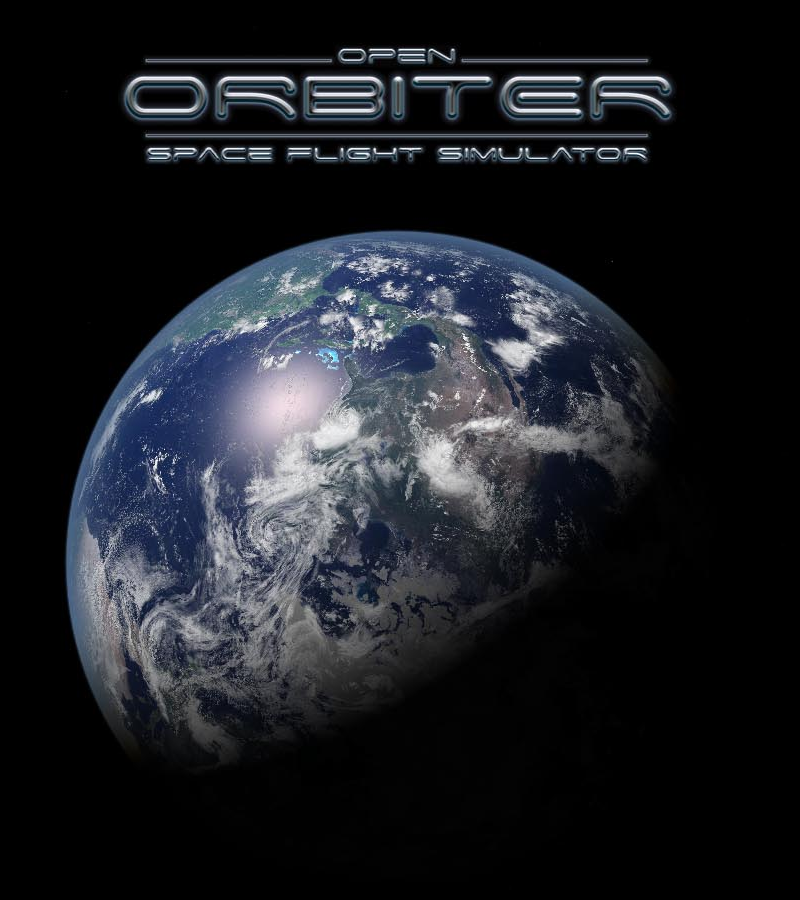
\includegraphics[width=0.75\textwidth]{..//orbiterlogo.png}
\vspace{2.0cm}

\textsc{\LARGE Orbiter Developer Manual}

\end{center}
\end{titlepage}


\newpage
\pagenumbering{roman}

\tableofcontents
\newpage

\pagenumbering{arabic}

\newpage
\subfile{INTRODUCTION}
\newpage
\subfile{FLOW}
\newpage
\subfile{ORBITS}
\newpage
\subfile{SCENARIO}
\newpage
\subfile{CONFIG}
\newpage
\subfile{PLANETS}
\newpage
\subfile{NEW_SPACECRAFT}
\newpage
\subfile{VESSEL_CFG}
\newpage
\subfile{SPACECRAFT}
\newpage
\subfile{MESH}
\newpage
\subfile{SURFACES}
\newpage
\subfile{GRAPHICS_CLIENT}
\newpage
\subfile{PUBLISH}
\newpage
\subfile{SCN_EDITOR}
\newpage
\subfile{SOURCES}
\newpage
\bibliography{REFERENCES}

\end{document}